\documentclass[tikz,border=8pt]{standalone}
\usetikzlibrary{arrows.meta,calc}
\begin{document}
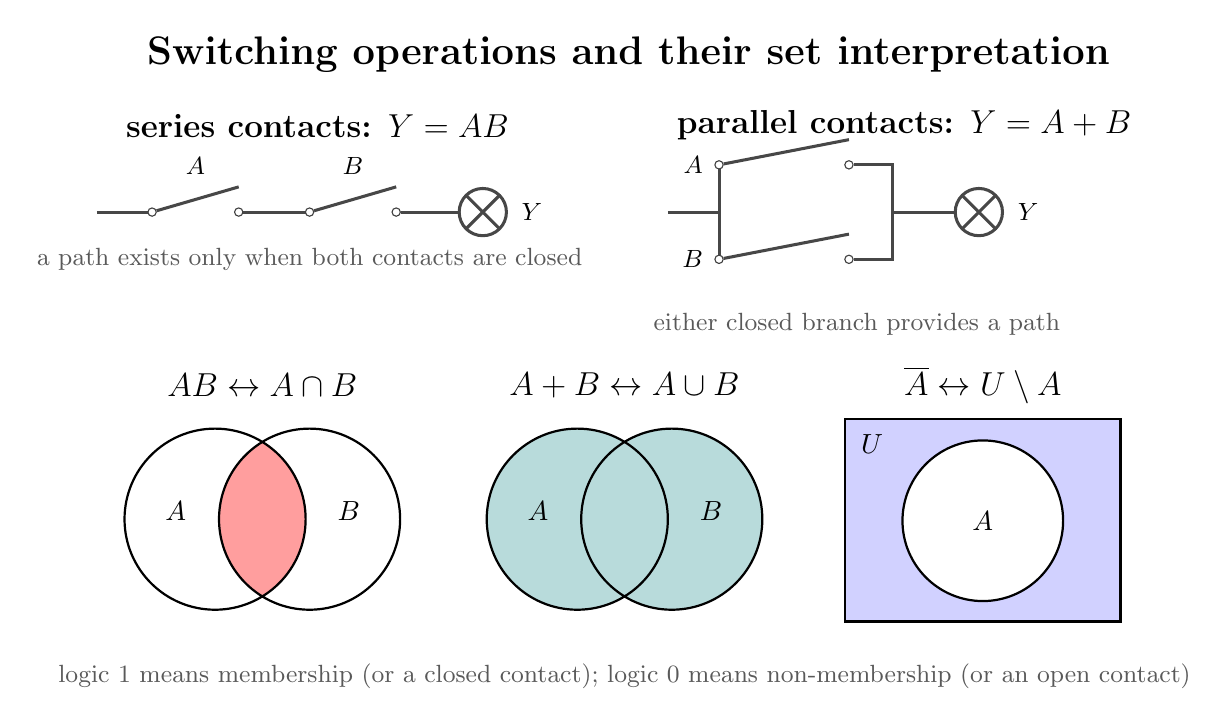
\begin{tikzpicture}[
  font=\sffamily,
  wire/.style={draw=black!72,line width=1.1pt},
  contact/.style={circle,draw=black!75,fill=white,inner sep=0pt,minimum size=3pt},
  label/.style={font=\small},
  title/.style={font=\bfseries\large}
]
\node[font=\bfseries\Large] at (7.2,8.35) {Switching operations and their set interpretation};

% Series contacts: closed A AND closed B completes the path.
\node[title] at (3.25,7.45) {series contacts: $Y=AB$};
\draw[wire] (.45,6.35) -- (1.15,6.35);
\node[contact] (a1) at (1.15,6.35) {};
\node[contact] (a2) at (2.25,6.35) {};
\draw[wire] (a1) -- ([yshift=.32cm]a2.center);
\node[label,above] at (1.7,6.7) {$A$};
\draw[wire] (a2) -- (3.15,6.35);
\node[contact] (b1) at (3.15,6.35) {};
\node[contact] (b2) at (4.25,6.35) {};
\draw[wire] (b1) -- ([yshift=.32cm]b2.center);
\node[label,above] at (3.7,6.7) {$B$};
\draw[wire] (b2) -- (5.05,6.35);
\draw[wire] (5.35,6.35) circle (.30);
\draw[wire] (5.14,6.14) -- (5.56,6.56) (5.14,6.56) -- (5.56,6.14);
\node[label,right] at (5.72,6.35) {$Y$};
\node[label,text=black!65] at (3.15,5.75) {a path exists only when both contacts are closed};

% Parallel contacts: either closed branch completes the path.
\node[title] at (10.7,7.45) {parallel contacts: $Y=A+B$};
\draw[wire] (7.7,6.35) -- (8.35,6.35) -- (8.35,6.95);
\draw[wire] (8.35,6.35) -- (8.35,5.75);
\node[contact] (pa1) at (8.35,6.95) {};
\node[contact] (pa2) at (10.0,6.95) {};
\draw[wire] (pa1) -- ([yshift=.32cm]pa2.center);
\node[label,left] at (8.27,6.95) {$A$};
\node[contact] (pb1) at (8.35,5.75) {};
\node[contact] (pb2) at (10.0,5.75) {};
\draw[wire] (pb1) -- ([yshift=.32cm]pb2.center);
\node[label,left] at (8.27,5.75) {$B$};
\draw[wire] (pa2) -- (10.55,6.95) -- (10.55,6.35);
\draw[wire] (pb2) -- (10.55,5.75) -- (10.55,6.35) -- (11.35,6.35);
\draw[wire] (11.65,6.35) circle (.30);
\draw[wire] (11.44,6.14) -- (11.86,6.56) (11.44,6.56) -- (11.86,6.14);
\node[label,right] at (12.02,6.35) {$Y$};
\node[label,text=black!65] at (10.1,4.92) {either closed branch provides a path};

% Venn diagrams: intersection, union and complement.
\node[title] at (2.55,4.15) {$AB\leftrightarrow A\cap B$};
\begin{scope}
  \clip (1.95,2.45) circle (1.15);
  \fill[red!38] (3.15,2.45) circle (1.15);
\end{scope}
\draw[thick] (1.95,2.45) circle (1.15) (3.15,2.45) circle (1.15);
\node at (1.45,2.55) {$A$}; \node at (3.65,2.55) {$B$};

\node[title] at (7.15,4.15) {$A+B\leftrightarrow A\cup B$};
\fill[teal!28] (6.55,2.45) circle (1.15);
\fill[teal!28] (7.75,2.45) circle (1.15);
\draw[thick] (6.55,2.45) circle (1.15) (7.75,2.45) circle (1.15);
\node at (6.05,2.55) {$A$}; \node at (8.25,2.55) {$B$};

\node[title] at (11.7,4.15) {$\overline A\leftrightarrow U\setminus A$};
\fill[blue!18] (9.95,1.15) rectangle (13.45,3.72);
\fill[white] (11.7,2.43) circle (1.02);
\draw[thick] (9.95,1.15) rectangle (13.45,3.72);
\draw[thick] (11.7,2.43) circle (1.02);
\node at (11.7,2.43) {$A$};
\node[anchor=north west] at (10.03,3.65) {$U$};

\node[font=\small,text=black!65] at (7.15,.45)
  {logic 1 means membership (or a closed contact); logic 0 means non-membership (or an open contact)};
\end{tikzpicture}
\end{document}
